\section{Стимулы агента с причинной точки зрения}

\subsection{Ключевые идеи}

Статья~\cite{everitt2021agentincentives} формирует единый причинный подход к анализу стимулов, которые возникают 
у агента при максимизации полезности. Среда задаётся структурной причинной моделью, 
а взаимодействие агента со средой — причинной диаграммой влияния. 
Объединяя эти две конструкции в структурную модель с влиянием, авторы получают 
формализм, позволяющий описывать политику агента и рассматривать контрфактуальные 
вмешательства.

В рамках этой модели можно определить четыре типа стимулов, возникающих у оптимального агента:

\begin{itemize}
    \item \emph{ценность информации} — насколько агенту выгодно наблюдать переменную;
    \item \emph{ценность контроля} — насколько полезно уметь управлять переменной;
    \item \emph{реакционный стимул} — будет ли решение агента меняться при изменении переменной;
    \item \emph{инструментальный контрольный стимул} — будет ли агент стремиться воздействовать на переменную через своё действие.
\end{itemize}

Главная идея статьи состоит в том, что все эти свойства можно определить, 
опираясь только на графовую структуру причинных зависимостей. Авторы дают 
звуковые и полные критерии, основанные на d-разделимости, которые позволяют 
предсказывать стимулы ещё до реализации системы. Благодаря этому можно заранее 
выявить ситуации, в которых оптимальный агент станет, например, использовать 
чувствительные признаки или манипулировать пользователем.

\subsection{Математическое описание метода}

Структурная причинная модель с влиянием представляется четверкой
\begin{equation}
    M = \langle G, E, F, P \rangle,
\end{equation}
где $G$~-- причинная диаграмма влияния, описывающая структуру зависимостей между переменными;  
$E$~-- набор экзогенных переменных, отвечающих за всю случайность модели;  
$F$~-- набор структурных функций, задающих значения всех переменных, кроме решения;  
$P$~-- распределение над экзогенными переменными.  

Эта формализация позволяет рассматривать модель как абстрактное "окружение" для агента.  
Для узла решения $D$ родители $Pa_D$ представляют собой наблюдения, доступные агенту,  
а дополнительная экзогенная переменная $E_D$ задаёт его внутреннюю случайность.  
Политика агента записывается как
\begin{equation}
    D = \pi(Pa_D, E_D).
\end{equation}

После фиксации конкретной политики $\pi$ узел решения перестаёт быть особым,  
и модель превращается в обычную структурную причинную модель.  
Это даёт возможность использовать стандартные операции интервенций и контрфактуалов.

Полезность определяется как сумма всех узлов $U_i \in \mathcal{U}$:
\begin{equation}
    U = \sum_{U_i \in \mathcal{U}} U_i,
\end{equation}
а максимальная ожидаемая полезность агента в модели $M$ задаётся выражением
\begin{equation}
    V^*(M) = \max_{\pi} \mathbb{E}_{\pi}[U].
\end{equation}

\paragraph{Ценность информации.}  
Чтобы оценить, полезно ли агенту наблюдать некоторую переменную $X$,  
рассматривается модель, в которой агент получает дополнительную дугу $X \to D$.  
Разность максимальных полезностей в модифицированной и исходной моделях:
\begin{equation}
    V^*(M_{X \to D}) - V^*(M)
\end{equation}
определяет \emph{ценность информации}.  
Если
\begin{equation}
    V^*(M_{X \to D}) > V^*(M),
\end{equation}
то переменная действительно помогает агенту принимать более выгодные решения.  

Графовый критерий использует d-связность: переменная $X$ должна быть d-связана  
с потомками решения среди узлов полезности при условии на остальные наблюдения.  
Формально:
\begin{equation}
    X \not\!\perp\!\!\!\perp U_D \mid \bigl(Pa_D \cup \{D\} \setminus \{X\}\bigr),
\end{equation}
где $U_D$~-- узлы полезности, зависящие от решения.  


\paragraph{Реакционный стимул.}  
Здесь рассматривается вопрос: \emph{будет ли агент менять своё решение,  
если некоторое значение $X$ контрфактуально изменится?}  
Для этого используется величина $D_x$,  
которая обозначает решение в мире, где проводится действие $do(X = x)$.  

Если существует значение $x$, такое что для некоторой реализации экзогенных 
переменных $\varepsilon$
\begin{equation}
    D_x(\varepsilon) \neq D(\varepsilon)
\end{equation}
и это верно для всех оптимальных политик,  
то говорят, что у агента существует реакционный стимул на $X$.

Графовая проверка проводится в минимальной редукции (без нематериальных наблюдений).  
Реакционный стимул присутствует тогда и только тогда,  
когда в этой редукции есть ориентированный путь от $X$ к $D$.


\paragraph{Ценность контроля.}  
Здесь рассматривается, выгодно ли агенту иметь возможность напрямую управлять переменной $X$.
Для этого в модели заменяется её структурная функция $f_X$ на произвольную $g_X$,  
совместимую с её родителями и экзогенным шумом.  
С новой функцией полезность записывается как $U^{g_X}$.  
Положительная ценность контроля означает:
\begin{equation}
    \max_{\pi, g_X} \mathbb{E}_{\pi}[U^{g_X}] > \max_{\pi} \mathbb{E}_{\pi}[U].
\end{equation}

В минимальной редукции это возможно тогда и только тогда,  
когда от $X$ существует ориентированный путь к какому-либо узлу полезности.  

\paragraph{Инструментальный контрольный стимул.}  
В отличие от предыдущего случая, здесь рассматривается не прямой контроль переменной,  
а тот контроль, который возникает через действие агента.  
Пусть $X_d$ обозначает значение $X$ в мире, где действие принудительно установлено в $d$.  
Полезность в таком мире обозначается $U^{X_d}$.

Стимул присутствует, если в некотором контексте наблюдений $pa_D$ выполняется
\begin{equation}
    \mathbb{E}\bigl[U^{X_d} \mid pa_D\bigr] \neq \mathbb{E}\bigl[U \mid pa_D\bigr]
\end{equation}
для некоторого действия $d$ и всех оптимальных политик.

Авторы показывают, что это происходит тогда и только тогда,  
когда в исходной причинной диаграмме влияния есть ориентированный путь
\begin{equation}
    D \rightsquigarrow X \rightsquigarrow U,
\end{equation}
то есть решение влияет на переменную $X$, а она — на полезность.  

Такой путь означает, что агент может повысить полезность,  
если выберет действие, изменяющее $X$.  
Именно это и является инструментальным контролем.


\subsection{Алгоритм}

Процесс можно представить как последовательность шагов, каждый из которых 
отвечает на свой вопрос о поведении оптимального агента.

\begin{enumerate}
    \item Построение диаграммы влияния. 
    Сначала формируется граф, в котором указываются все переменные среды, 
    узел решения и узлы полезности, а также отмечается, какие переменные 
    доступны агенту для наблюдения.
    
    \item Получение минимальной редукции.  
    Затем из диаграммы удаляются наблюдения, которые никак не могут повлиять 
    на максимальную ожидаемую полезность.

    \item Проверка ценности информации. 
    Чтобы понять, может ли агент выиграть от наблюдения переменной $X$, 
    в диаграмму мысленно добавляют дугу $X \to D$. Далее проверяют, 
    появляется ли d-связность между $X$ и потомками решения среди узлов 
    полезности. Если такая связь возникает, то наблюдение $X$ действительно 
    может улучшить ожидаемую награду.
    
    \item Проверка реакционного стимула. 
    Реакционный стимул выявляется, когда в минимальной редукции существует 
    ориентированный путь от переменной $X$ к решению $D$. Это означает, 
    что изменение $X$ способно изменить оптимальную политику~-- даже если агент 
    не управляет этой переменной напрямую.
    
    \item Проверка ценности контроля. 
    Далее проверяется, существует ли путь от $X$ к узлу полезности. Если он есть, 
    значит, управление $X$ потенциально может повысить ожидаемую полезность. 
    
    \item Проверка инструментального контрольного стимула.  
    Наконец, рассматривается структура путей от решения к переменной. Если 
    существует цепочка $D \rightsquigarrow X \rightsquigarrow U$, то агент 
    может повысить награду, воздействуя на $X$ именно через своё действие. 
    
    Это и есть инструментальный контрольный стимул — ситуация, когда управление 
    переменной становится полезным инструментом достижения цели.
\end{enumerate}

\subsection{Наборы данных (сценарии)}

В статье рассматриваются два теоретических сценария, которые играют роль 
наборов данных.

Первый сценарий относится к \emph{прогнозированию оценок студентов}. В качестве 
переменных рассматриваются раса абитуриента, школа, в которой он учился, 
уровень полученного школьного образования и итоговая оценка в университете. 
Модель предполагает, что качество образования зависит от школы, школа в 
среднем связана с расой, а пол не влияет на успеваемость. Решение агента 
состоит в предсказании будущей оценки студента, а полезность отражает точность 
предсказания. 

На рисунке~\ref{fig:decision_problems} слева показана 
причинная диаграмма влияния для этого сценария, а 
на рисунке~\ref{fig:response_incentives} показано, как меняются пути стимулов 
при наличии или отсутствии информации о школе.

\begin{figure}
    \centering
    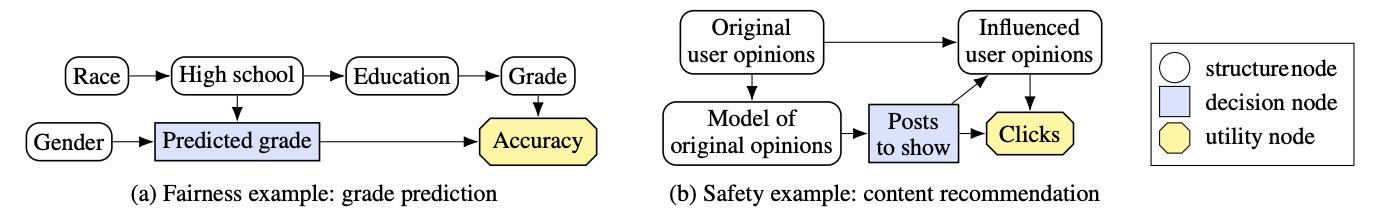
\includegraphics[width=\linewidth]{images/fig1_decision_problems.png}
    \caption{Диаграммы причинно-следственных связей для прогнозирования оценок 
    и рекомендаций по содержанию.}
    \label{fig:decision_problems}
\end{figure}


\begin{figure}
    \centering
    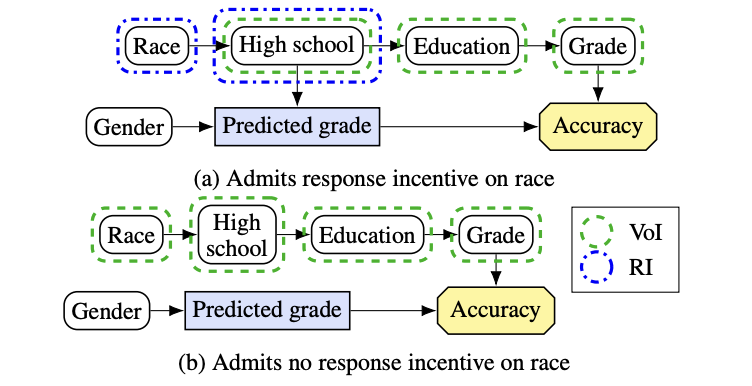
\includegraphics[width=0.85\linewidth]{images/fig3_response_incentives.png}
    \caption{Реакция и информационные стимулы в сценарии прогнозирования оценок.}
    \label{fig:response_incentives}
\end{figure}

Второй сценарий посвящён \emph{рекомендательной системе}. Здесь рассматриваются 
исходные взгляды пользователя, выбираемые посты и клики пользователя, 
а также изменённые взгляды после просмотра контента. 
Решение агента~-- какие посты показывать, полезность определяется числом кликов. 
В этом сценарии ключевой вопрос~-- будет ли агент стремиться манипулировать 
взглядами пользователя для повышения предсказуемости или частоты кликов. 

Структура причинной диаграммы для этого сценария изображена справа на 
рисунке~\ref{fig:decision_problems}, а влияние различных формулировок 
цели на стимулы к манипуляции показано на рисунке~\ref{fig:control_incentives}.

\begin{figure}
    \centering
    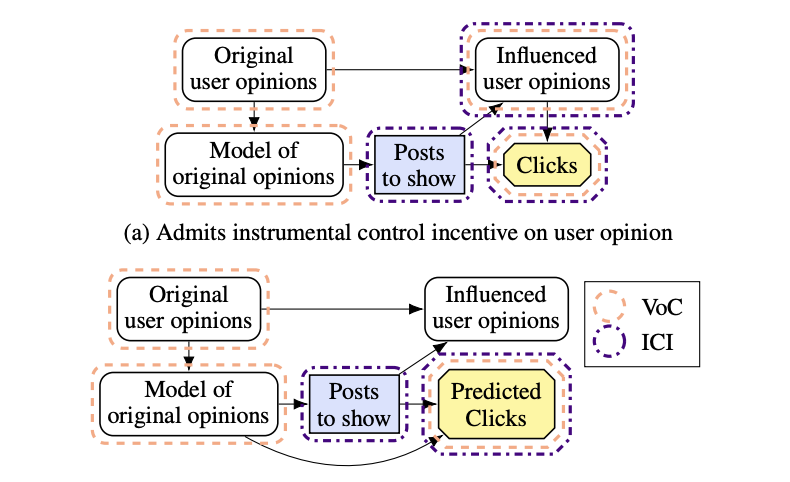
\includegraphics[width=0.85\linewidth]{images/fig4_control_incentives.png}
    \caption{Значение контроля и инструментальных стимулов для контроля 
    в сценарии рекомендаций по содержанию.}
    \label{fig:control_incentives}
\end{figure}


\subsection{Метрики}

Основной количественной характеристикой, используемой в статье, является 
ожидаемая суммарная полезность агента при фиксированной политике. 
Явной формулы авторы не приводят, поэтому ниже используется собственное 
обозначение, согласованное с основной моделью. Для политики $\pi$ определим 
её ожидаемую полезность как
\begin{equation}
    V(\pi \mid M) = \mathbb{E}_{\pi}[U],
\end{equation}
где математическое ожидание берётся по распределению, задаваемому 
структурной моделью $M$ вместе с политикой $\pi$, а $U$ есть сумма всех узлов полезности.

Максимальная достижимая полезность в модели выражается как
\begin{equation}
    V^*(M) = \max_{\pi} V(\pi \mid M).
\end{equation}

Для оценки \emph{ценности информации} переменной $X$ можно ввести выражение
\begin{equation}
    \Delta_{\mathrm{info}}(X) = V^*(M_{X \to D}) - V^*(M),
\end{equation}
где $M_{X \to D}$ обозначает модель, в которую добавлена дуга $X \to D$. 
Если $\Delta_{\mathrm{info}}(X) > 0$, то наблюдение $X$ способно улучшить оптимальное поведение.

Аналогично, для \emph{ценности контроля} определим
\begin{equation}
    \Delta_{\mathrm{ctrl}}(X) = 
        \max_{\pi,\, g_X}\mathbb{E}_{\pi}[U^{g_X}] 
        - 
        V^*(M),
\end{equation}
где $U^{g_X}$ соответствует полезности в модели, в которой структурная функция 
узла $X$ заменена на произвольную функцию $g_X$, согласованную с графом. 
Если $\Delta_{\mathrm{ctrl}}(X) > 0$, то управление переменной может повысить 
ожидаемую награду.


\subsection{Модели}

Статья опирается на три теоретические модели, каждая из которых описывает 
свою сторону взаимодействия агента со средой.

\begin{itemize}
    \item \emph{Структурная причинная модель (SCM).}  
    Эта модель задаёт причинно-следственные зависимости между переменными 
    через набор детерминированных функций и экзогенных факторов. Она позволяет 
    строго определять вмешательства и контрфактуальные значения, что делает 
    её подходящей основой для анализа поведения агента.
    
    \item \emph{Причинная диаграмма влияния (CID).}  
    В этой диаграмме выделяются наблюдаемые переменные, узел решения и узлы 
    полезности. CID показывает, какую информацию получает агент перед выбором 
    действия и какие последствия это действие имеет.

    \item \emph{Структурная модель с влиянием (SCIM).}  
    Эта модель объединяет SCM и CID: причинная диаграмма определяет 
    информационную структуру, а структурные функции описывают динамику всех 
    переменных, кроме решения. Решение задаётся политикой агента. 
\end{itemize}

На рисунке~\ref{fig:scim} показано, как SCIM используется для сценария 
рекомендаций контента: базовая модель, модель после фиксации политики и 
модель с вложенным контрфактуалом, описывающим влияние гипотетического выбора постов.

\begin{figure}
    \centering
    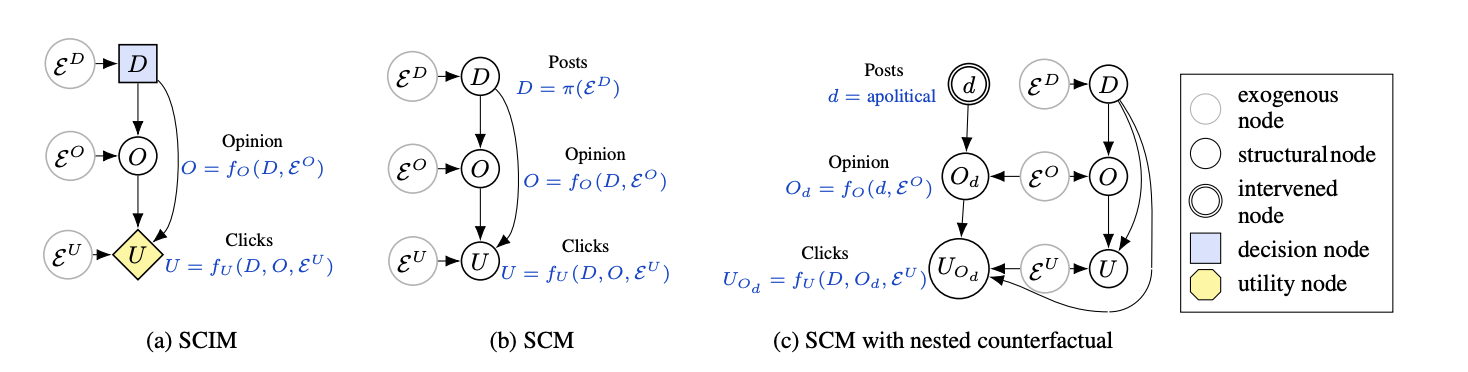
\includegraphics[width=\linewidth]{images/fig2_scim_interventions.png}
    \caption{SCIM, индуцированный SCM и вложенные контрфакты в сценарии рекомендаций по содержанию.}
    \label{fig:scim}
\end{figure}
